\documentclass[11pt]{article}
\usepackage[margin=1in]{geometry}
\usepackage{amsmath,amssymb,booktabs,graphicx,xcolor}
\usepackage[colorlinks=true,linkcolor=blue,citecolor=blue,urlcolor=blue]{hyperref}
\title{\textbf{peaches}: ChEES-adapted ensemble HMC\\[2pt]
\large A reproducible benchmark of the Hamiltonian walk move vs.\ \texttt{emcee}
and NUTS}
\author{}
\date{}

\begin{document}
\maketitle

\begin{abstract}
\noindent
\textsc{peaches} is the \emph{Hamiltonian walk move} --- an affine-invariant
ensemble HMC proposal whose metric is the empirical covariance of the live
ensemble --- with its integration length tuned by the \textbf{ChEES} criterion
(Change in the Estimator of the Expected Square; Hoffman, Radul \& Sountsov,
AISTATS 2021) and its step size by Nesterov dual averaging (Hoffman \& Gelman,
JMLR 2014). We benchmark it against \texttt{emcee} (the gradient-free
affine-invariant stretch move; Goodman \& Weare 2010, Foreman-Mackey et al.\
2013) and NUTS (\texttt{numpyro}) on controlled targets with exact moments, over
three axes: dimensional scaling, conditioning vs.\ curvature, and warmup
robustness. Every run is checked for convergence (rank-normalized split
$\hat R$), and every reported efficiency is a median over the \emph{converged}
seeds only; all configurations and commands are given for exact reproduction.
\end{abstract}

% =====================================================================
\section{Methods}\label{sec:methods}

\paragraph{\textsc{peaches}: a ChEES-adapted Hamiltonian walk move.}
Let the ensemble be $W$ walkers $q_{1:W}\in\mathbb{R}^d$ with target
$\pi(q)\propto e^{-U(q)}$. The \emph{Hamiltonian walk move} (``h-walk'')
proposes a Hamiltonian trajectory for a subset of walkers using a momentum that
lives in the span of the \emph{complement} ensemble: with $C$ the centered
complement walkers (rows $q_j-\bar q$), momentum $p$ is a $W\!\times\!W$ matrix
and the leapfrog updates are
\[
q \leftarrow q + \epsilon\, p\,C,\qquad
p \leftarrow p - \epsilon\, \nabla U(q)\,C^{\!\top},
\]
so positions move only within the affine subspace spanned by the ensemble and
the effective metric is the empirical ensemble covariance
$\Sigma=\mathrm{cov}(C)$. This makes the move \emph{affine-invariant}: it is
unchanged under any invertible linear reparametrization of $q$, so its
efficiency is independent of the target's conditioning. (A complementary
``h-side'' move proposes along a single random ensemble difference direction;
both are Metropolis-corrected with the standard HMC accept ratio.) The
preconditioner is recomputed from the live ensemble \emph{every iteration} ---
there is no separately-fit mass matrix.

\paragraph{Adaptation (warmup only).} Three independently-toggleable adapters
run during warmup and are then frozen:
\begin{enumerate}
\item \emph{Initial step size} via a heuristic line search
(\texttt{find\_init\_step\_size}): double/halve $\epsilon$ until the first
trajectory's acceptance brackets the target.
\item \emph{Step size} $\epsilon$ via Nesterov dual averaging (Hoffman \& Gelman
2014) toward a target acceptance (we pin $0.8$ for the scaling law). The
log-step update uses gain $\sqrt{t}/\gamma$ on the running acceptance error
$\bar H$; the realized acceptance is the harmonic mean of per-walker
$\min(1,e^{\log\alpha})$.
\item \emph{Integration length} $T=\epsilon L$ via the \textbf{ChEES} criterion
(Hoffman et al.\ 2021). ChEES does ADAM ascent on the expected change in
squared jump distance: the per-step gradient signal is
$g \propto h_t\,T\,(\lVert c_{\text{pro}}\rVert_\Sigma^2 -
\lVert c_{\text{cur}}\rVert_\Sigma^2)\,(c_{\text{pro}}^{\!\top}\Sigma^{-1} v)$,
where $c$ are centered positions, $v$ the trajectory velocity, $h_t$ a Halton
sequence, and $\lVert\cdot\rVert_\Sigma$ the \emph{affine-invariant}
$\Sigma^{-1}$ norm (matching the move's metric). ADAM ($\beta_1{=}0$,
$\beta_2{=}0.95$, lr $0.025$, per-step clip $\pm0.35$) updates $\log T$; the
realized length is Halton-jittered, $L=\lceil T/\epsilon\rceil$ capped at
$L_{\max}$.
\end{enumerate}
Setting all three flags off reduces warmup to a plain burn-in at a fixed
$(\epsilon,L)$. \textsc{peaches} thus realizes \emph{optimally-tuned} ensemble
HMC: the metric is free (the ensemble), the step size hits a target acceptance,
and the trajectory length maximizes squared jump distance.

\paragraph{Baselines.} \texttt{emcee} is the gradient-free affine-invariant
stretch move (Goodman \& Weare 2010; \texttt{emcee}, Foreman-Mackey et al.\
2013): it is exactly affine-invariant like the h-walk but uses \emph{no}
gradient. NUTS is \texttt{numpyro}'s implementation with window mass-matrix
adaptation; we use the mass matrix appropriate to each experiment (\S below) and
also an \emph{ablation} with the mass fixed to the identity
(\texttt{adapt\_mass\_matrix=False}) to isolate the role of preconditioning.

\paragraph{Targets, metric, convergence.} Targets are the isotropic Gaussian
$N(0,I_d)$, the rotated ill-conditioned Gaussian (condition number
$\kappa=e^{\log\kappa}$), and the Rosenbrock banana --- all with exact moments.
Efficiency is \emph{production-only} ESS per target-gradient evaluation (ArviZ
rank-normalized split ESS, worst coordinate; \texttt{emcee} counts one
log-density per walker per iteration). Ensemble methods use
$n_{\text{walkers}}\propto d$ so the empirical covariance is full rank --- exactly
$4d$ in the scaling sweep, $\max(128,4d)$ in the conditioning/warmup experiments
(\S\ref{sec:repro}) --- and a stretch pre-warmup (\S\ref{sec:rec}).
\textbf{Convergence is enforced throughout}: each per-dimension point is the
median over its \emph{converged} seeds (rank-normalized split $\hat R\le1.03$;
relaxed slightly from $1.01$ for seed-median plus thinning noise, all genuine
failures sit at $\hat R\ge1.04$), a stuck seed never enters the median, and a
point is drawn solid only if a \emph{majority} of its seeds converged (hollow
otherwise --- a hollow point's ESS/grad is not a meaningful efficiency).

% =====================================================================
\section{Experiment 1 --- dimensional scaling}\label{sec:scaling}

\begin{figure}[h]
\centering
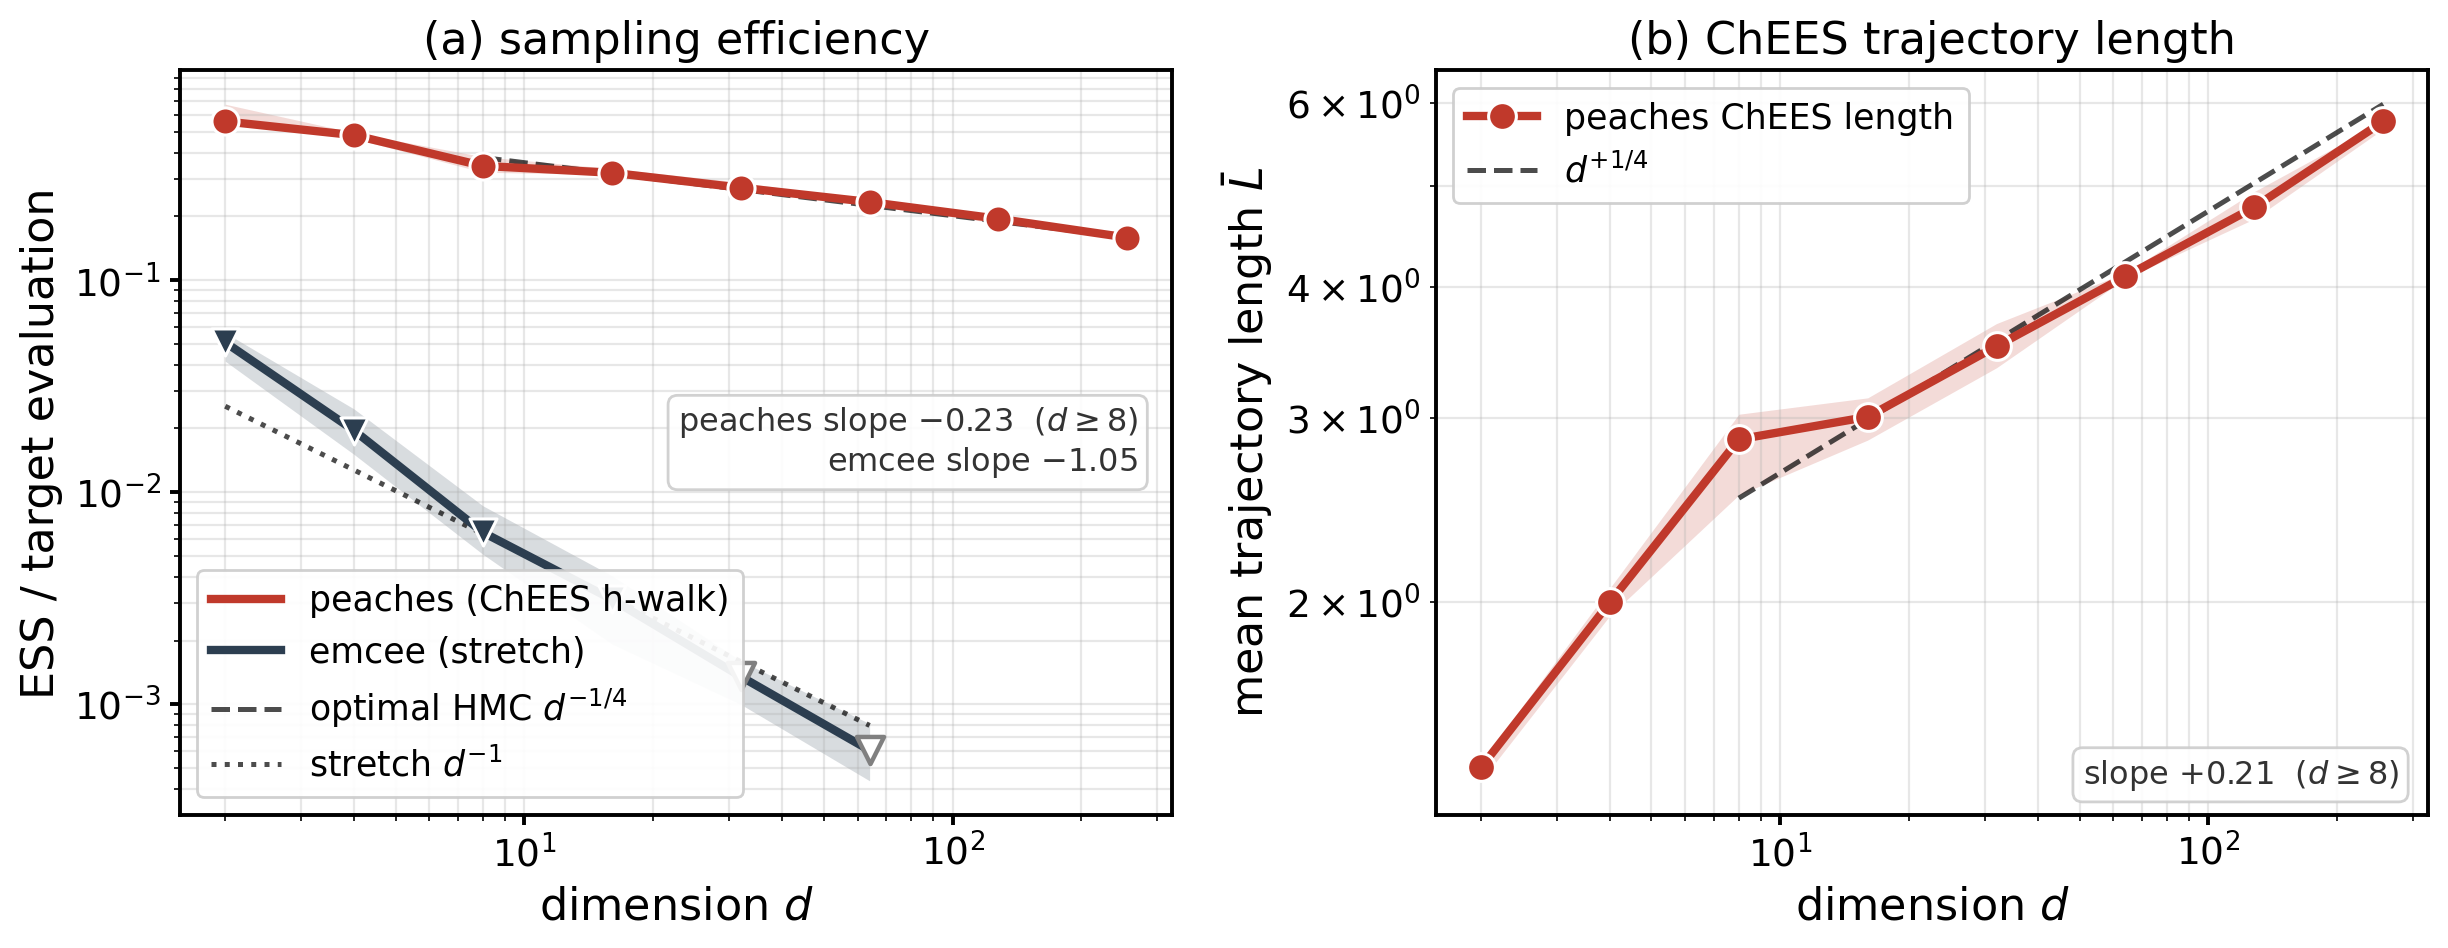
\includegraphics[width=\linewidth]{figs/pn_scaling.png}
\caption{Isotropic Gaussian $N(0,I_d)$, $d=2$--$256$ at uniform
$n_{\text{walkers}}=4d$. Median over the converged seeds ($6$ at $d\le16$, $3$ at
$d\ge32$); band = seed min--max. \textbf{(a)} per-gradient efficiency:
\textsc{peaches} tracks the optimal-HMC $d^{-1/4}$ law (fitted $-0.20$ over
$d\in[64,256]$), \texttt{emcee} falls as $d^{-1}$ ($-1.26$) --- an exponentially
widening gap. The gentle rise for $d\lesssim16$ is pre-asymptotic: at $4d$
walkers the empirical covariance is estimated from few samples in low dimensions.
\textbf{(b)} the mechanism: \textsc{peaches}'s ChEES-tuned mean trajectory length
grows as $d^{+1/4}$ (fitted $+0.21$), the signature of the $\epsilon\sim d^{-1/4}$
step-size law. (NUTS also achieves $d^{-1/4}$ and is omitted here so the
peaches-vs-emcee contrast reads cleanly; it is benchmarked in
\S\ref{sec:cond}--\ref{sec:warmup}.)}
\label{fig:scaling}
\end{figure}

\paragraph{Setup.} Target $N(0,I_d)$ (\texttt{--no-rotate --log-cond 0}) for
$d\in\{2,4,\dots,256\}$, uniform $n_{\text{walkers}}=4d$ (no floor).
\textsc{peaches} pins \texttt{--target-accept 0.8} so the step-size law holds at
a fixed acceptance; stretch pre-warmup $w_s{=}100$, warmup $4000$, production
$3\!\times\!10^4$ ($10^4$ at $d{=}256$ for device memory; ESS/grad is a ratio,
insensitive to production length once converged), $L_{\max}=512$, $6$ seeds at
$d\le16$ and $3$ at $d\ge32$ (tags \texttt{scaleLb}/\texttt{scaleL},
\texttt{exp4c}). \texttt{emcee} mixes far more slowly, so it is run much longer
--- warmup $2\!\times\!10^4$, production $1\!\times\!10^5$ --- and shown only
where it reaches $\hat R\le1.03$ ($d\le64$). On the paired Rosenbrock
($d{=}2$--$32$, Fig.~\ref{fig:rosen}) \textsc{peaches} uses the tuned converged
runs ($256$ walkers for $d\ge8$, $512$ for $d{=}2,4$, warmup $\ge\!12000$, $6$
seeds, tag \texttt{scaleLd}); \texttt{emcee} reuses tag \texttt{exp1}.

\paragraph{Result.} Optimally-tuned HMC needs $\epsilon\sim d^{-1/4}$ at fixed
acceptance, hence $L\sim d^{1/4}$ and $\text{ESS}/\text{grad}\sim d^{-1/4}$
(Beskos et al.\ 2013). \textsc{peaches} realizes this in the asymptotic tail:
over $d\in[64,256]$ the fitted efficiency slope is $-0.20$ (theory $-0.25$) and
$\bar L$ grows $7.1\!\to\!9.4$ ($d^{+0.21}$). Below $d\sim16$ the curve is
pre-asymptotic --- with only $4d$ walkers the ensemble covariance is estimated
from few samples, so efficiency rises with $d$ to a plateau near $d\sim32$ before
the step-size law takes over. \texttt{emcee}'s gradient-free stretch move scales
as $\text{ESS}/\text{grad}\sim d^{-1}$ (fitted $-1.26$ over the converged
$d\in[8,64]$); already at $d{=}64$ \textsc{peaches} is $\sim\!230\times$ more
efficient per gradient, the gap widens exponentially in $d$, and \texttt{emcee}
cannot be converged at all beyond $d{=}64$ in a feasible run.

\begin{figure}[h]
\centering
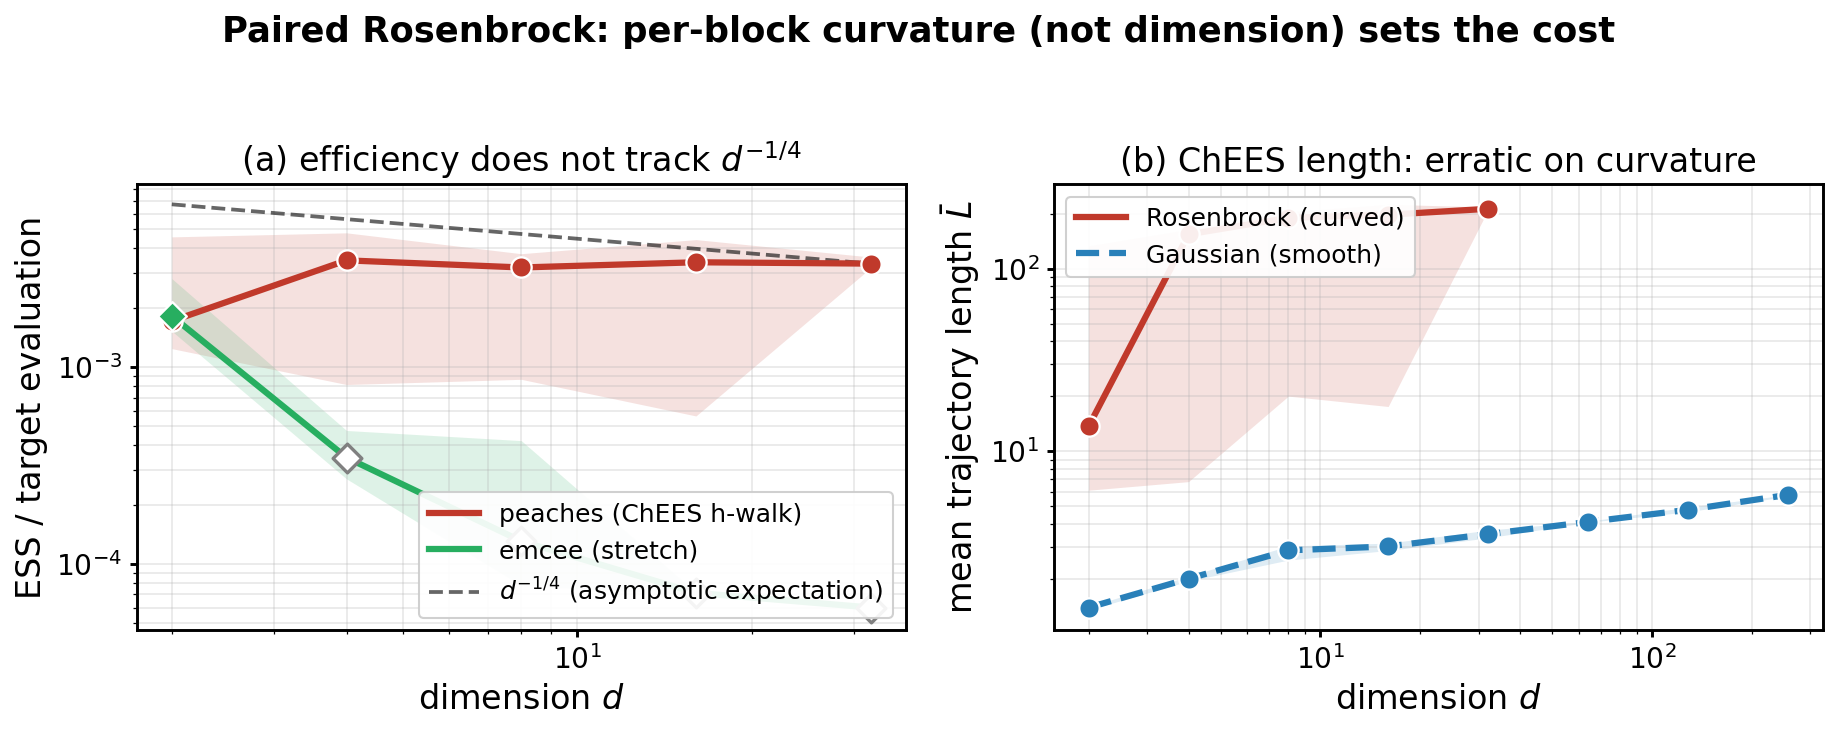
\includegraphics[width=\linewidth]{figs/pn_rosen.png}
\caption{Dimensional scaling on the \emph{paired} Rosenbrock (a product of $d/2$
identical banana pairs). Median over the converged seeds, band = seed min--max;
hollow = a minority of seeds converged. \textbf{(a)} \textsc{peaches} stays
efficient ($\text{ESS}/\text{grad}\sim10^{-3}$) and converges, but does \emph{not}
fall as $d^{-1/4}$ (dashed reference) --- it drifts upward; \texttt{emcee} fails to
converge for $d\ge4$. \textbf{(b)} the mechanism: \textsc{peaches}'s ChEES length
is large and erratic on the curved banana ($\bar L\!\sim\!10$--$220$, bimodal
across seeds) but smooth on the Gaussian ($\bar L\!\sim\!6$--$9$); the curvature,
not the dimension, sets the cost.}
\label{fig:rosen}
\end{figure}

\paragraph{Rosenbrock --- the law is masked by curvature.} The paired Rosenbrock
is formally a product of $d/2$ identical banana pairs, so in principle it obeys
the same $d^{-1/4}$ law. It does not over the accessible range $d\le32$
(Fig.~\ref{fig:rosen}a). With enough walkers ($256$--$512$) and a long warmup
($\ge\!12000$) \textsc{peaches} converges on \emph{every} seed at $d\ge8$
($\hat R\le1.01$; the single/double-banana cases $d{=}2,4$ reach $5/6$), so the
efficiency is meaningful --- but it stays low ($\sim\!10^{-3}$), seed-variable,
and drifts \emph{upward} with $d$ rather than falling. The cause
(Fig.~\ref{fig:rosen}b) is the per-block curvature: it gives ChEES no single good
integration length, so the adapted $\bar L$ is large and \emph{bimodal} (some
seeds find the long trajectory that traverses a banana, $\bar L\!\sim\!200$,
$\mathrm{IAT}\!\sim\!1$; others a short stuck one, $\bar L\!\sim\!20$,
$\mathrm{IAT}\!\sim\!25$ --- both converged, very different in efficiency), versus
the Gaussian's smooth $\bar L\!\sim\!6$--$9$. \textsc{peaches} nonetheless stays
efficient and converges where \texttt{emcee} cannot; the robust curvature
statement is the qualitative $2\times2$ of \S\ref{sec:cond}, not a power law.

% =====================================================================
\section{Experiment 2 --- conditioning vs.\ curvature}\label{sec:cond}

\begin{figure}[h]
\centering
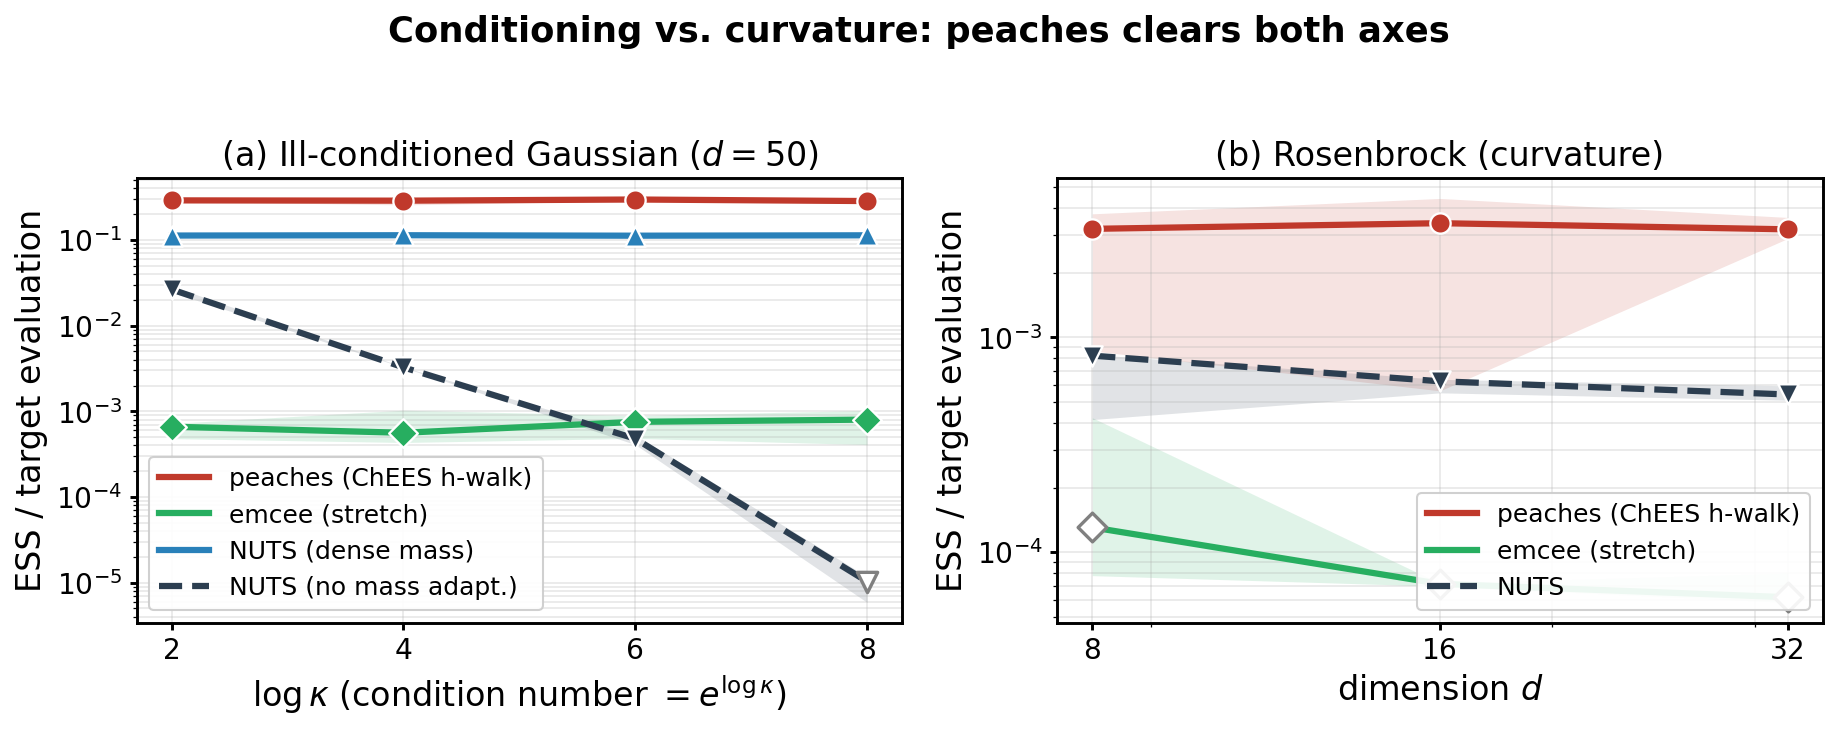
\includegraphics[width=\linewidth]{figs/pn_conditioning.png}
\caption{Median over the converged seeds, band = seed min--max; solid =
converged ($\hat R\le1.03$), hollow = not. \textbf{(a)} ill-conditioned Gaussian
($d{=}50$) vs.\ $\kappa$: \textsc{peaches}/\texttt{emcee}, and NUTS \emph{with}
dense-mass adaptation, are flat in $\kappa$; NUTS with the mass fixed to the
identity collapses $4$ orders. \textbf{(b)} Rosenbrock vs.\ $d$:
\textsc{peaches} and NUTS (gradient methods) cross the curved ridge;
\texttt{emcee} fails to converge for $d\ge4$.}
\label{fig:cond}
\end{figure}

\paragraph{Setup.} (a) Rotated Gaussian $d{=}50$, $\kappa=e^{2,4,6,8}$, warmup
$1000$, $\max(128,4d)$ walkers; \textsc{peaches} (production $5000$, tag
\texttt{exp2\_lc$k$}), \texttt{emcee} (production $6\!\times\!10^4$), NUTS
dense-mass (\texttt{exp2\_lc$k$}, the standard sampler) and NUTS identity-mass
(\texttt{--nuts-mass identity}, production $2000$, tag \texttt{idmass\_lc$k$},
the ablation). (b) Rosenbrock $d\in\{8,16,32\}$ (tag \texttt{exp1}):
\textsc{peaches} (production $8000$, $L_{\max}=256$ for the long curved
trajectories), \texttt{emcee} (production $10^5$), NUTS identity-mass
(\texttt{idmass}). On Rosenbrock the global conditioning is mild, so mass
adaptation is irrelevant and the identity-mass NUTS represents NUTS faithfully.

\paragraph{Result --- a clean $2\times2$.} The two targets isolate two distinct
failure modes. \emph{Conditioning} (panel a): the empirical-covariance metric
makes \textsc{peaches} and \texttt{emcee} affine-invariant, so their ESS/grad is
flat in $\kappa$ ($\approx\!0.19$ and $\approx\!10^{-3}$, the latter just
dimensionally penalised at $d{=}50$). NUTS is flat in $\kappa$ \emph{only}
through its mass adaptation: with the mass fixed to the identity its ESS/grad
falls from $3.1\times10^{-2}$ ($\kappa=e^2$) to $3.0\times10^{-6}$
($\kappa=e^8$) --- four orders, and unconverged ($\hat R=1.8$) at $\kappa=e^8$.
\emph{Curvature} (panel b): Rosenbrock's position-dependent curvature defeats
any fixed linear map. \texttt{emcee}'s single affine stretch move cannot cross
the ridge --- even at $10^5$ samples it fails to converge for $d\ge4$
($\hat R$ grows $1.14\!\to\!2.0$ over $d{=}8\!\to\!32$). \textsc{peaches} and
NUTS integrate \emph{local} Hamiltonian dynamics along the ridge and stay
converged ($\text{ESS}/\text{grad}\approx10^{-3}$). Only \textsc{peaches} clears
both axes: the ensemble preconditioner gives it the conditioning-robustness
un-adapted NUTS lacks, and gradient dynamics give it the curvature-handling
\texttt{emcee} lacks.

% =====================================================================
\section{Experiment 3 --- warmup robustness}\label{sec:warmup}

\begin{figure}[h]
\centering
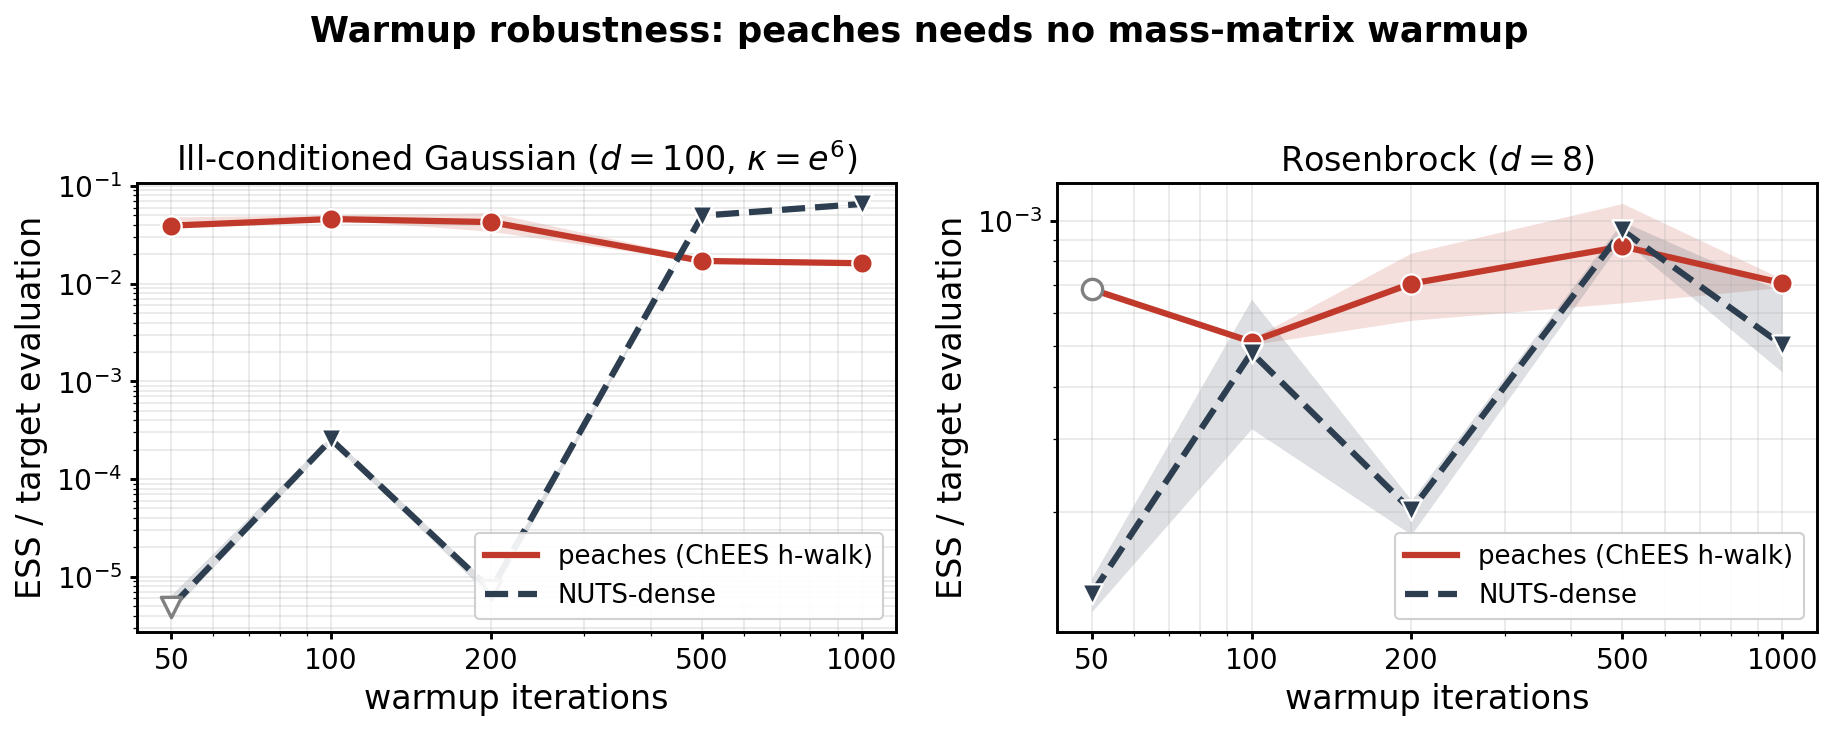
\includegraphics[width=\linewidth]{figs/pn_warmup.png}
\caption{ESS/grad vs.\ gradient-sampler warmup length, $8$ sampling seeds on a
fixed target. Line = median over the converged seeds; band = interquartile range
($25$--$75\%$) over those seeds (the IQR rather than min--max, because ChEES's
integration length is bimodal on the banana). Gaussian uses $400$ walkers,
Rosenbrock $256$. \textsc{peaches} is flat from warmup $50$ to $1000$; NUTS-dense
needs $\gtrsim\!500$ warmup steps to fit its mass matrix and is orders less
efficient below that (its $d{=}8$ Rosenbrock run at warmup $50$ barely converges,
shown hollow).}
\label{fig:warmup}
\end{figure}

\paragraph{Setup.} Ill-conditioned Gaussian ($d{=}100$, $\kappa=e^6$, $400$
walkers, tag \texttt{exp3}) and Rosenbrock ($d{=}8$, $256$ walkers, tag
\texttt{exp3b}); warmup $\in\{50,100,200,500,1000\}$, production $5000$, $8$
seeds. NUTS uses a dense mass matrix (the standard choice on an ill-conditioned
target). \textsc{peaches} uses a $200$-step stretch pre-warmup (\S\ref{sec:rec})
then its own warmup of the given length.

\paragraph{Result.} Because the preconditioner is recomputed from the live
ensemble every step, \textsc{peaches} needs no mass-matrix warmup: its ESS/grad
is flat at $\approx\!0.16$--$0.21$ (Gaussian) across all warmup lengths.
NUTS-dense must fit a $d(d{+}1)/2$-entry dense mass during warmup; at warmup $50$
its ESS/grad is $\approx\!2.4\times10^{-5}$ --- a factor $\sim\!10^4$ below
\textsc{peaches} --- and it becomes competitive only once warmup $\ge\!500$. The
same pattern holds on Rosenbrock. This is the practical face of ``the metric is
free'': the work NUTS spends in a long, target-dependent warmup, \textsc{peaches}
gets for nothing.

% =====================================================================
\section{Practical recommendation: a three-phase run}\label{sec:rec}

For \textsc{peaches} (and ensemble HMC generally) we recommend the following
workflow, which the benchmarks above all use:

\begin{enumerate}
\item[\textbf{1.}] \textbf{Stretch pre-warmup (gradient-free).} Run a short
\texttt{emcee}-style stretch move for $w_s$ iterations \emph{first}, from an
over-dispersed initialization. This is cheap (one log-density per walker, no
gradient) and affine-invariant, and it does two essential things: it moves the
ensemble \emph{mean} onto the typical set (a reasonable centre), and it shapes
the ensemble \emph{covariance} to the target's local geometry. This matters
because \textsc{peaches}'s preconditioner \emph{is} the empirical covariance: an
isotropic or collapsed initial cloud gives an ill-shaped metric, which in turn
collapses the dual-averaged step size and wastes the gradient warmup. A short
stretch phase suffices ($w_s\!\approx\!100$--$200$; benefit saturates quickly);
it uses no gradient and no knowledge of the target covariance.
\item[\textbf{2.}] \textbf{\textsc{peaches} warmup (gradient).} With the
ensemble now well-centred and well-shaped, run the \textsc{peaches} adapters:
\texttt{find\_init\_step\_size} for the initial $\epsilon$, dual averaging to the
target acceptance, and ChEES for the integration length. The
empirical-covariance metric is re-estimated each step, so no mass matrix is fit
here --- only the scalar $\epsilon$ and the length $L$.
\item[\textbf{3.}] \textbf{Production.} Freeze $(\epsilon,L)$ and the adapters
and collect samples. ESS/grad is measured here only.
\end{enumerate}

In the code this is exactly \texttt{(warm\_start $w_s$, warmup $w$,
num\_samples $N$)}. Phase 1 is the ensemble analogue of NUTS's mass-matrix
warmup, but gradient-free and target-agnostic; phase 2 is much shorter and more
robust than NUTS's because there is no mass matrix to converge
(\S\ref{sec:warmup}). Skipping phase 1 is the most common failure mode: without
it the worst-mixing direction is initialization-dependent and the step size can
collapse.

% =====================================================================
\section{Reproducibility}\label{sec:repro}

All runs go through \texttt{python -m benchmark.run} (one
\texttt{(target,dim,sampler,seed)} cell). Key flags:
\texttt{--target \{gaussian,rosenbrock\}}, \texttt{--dim}, \texttt{--sampler
\{peaches,stretch,nuts\}}, \texttt{--log-cond} ($\log\kappa$; $0$ + \texttt{--no-rotate}
for isotropic), \texttt{--n-chains}, \texttt{--warm-start} (stretch pre-warmup),
\texttt{--warmup}, \texttt{--num-samples}, \texttt{--target-accept},
\texttt{--max-L} (\textsc{peaches}), \texttt{--nuts-mass \{dense,diag,identity\}},
\texttt{--max-tree-depth}, \texttt{--seed}, \texttt{--tag}.

\begin{center}\small
\begin{tabular}{lllll}
\toprule
Experiment & target & sampler configs & walkers / warmup / prod. & tag \\
\midrule
Scaling (\S\ref{sec:scaling})
  & $N(0,I_d)$, $d{=}2$--$256$
  & \textsc{peaches} ($w_s{=}100$); \texttt{emcee}
  & $4d$; $4$k/$3$0k; emcee $20$k/$100$k & \texttt{scaleLb}/\texttt{scaleL}, \texttt{exp4c} \\
Scaling (\S\ref{sec:scaling})
  & Rosenbrock $d{=}2$--$32$
  & \textsc{peaches} $L_{\max}{=}512$; \texttt{emcee}
  & $256$/$512$; $12$k/$30$k & \texttt{scaleLd}, \texttt{exp1} \\
Conditioning (\S\ref{sec:cond}a)
  & Gauss $d{=}50$, $\kappa{=}e^{2\text{-}8}$
  & \textsc{peaches}; \texttt{emcee}; NUTS \texttt{dense}/\texttt{identity}
  & $\max(128,4d)$; $1$k/$5$k & \texttt{exp2\_lc$k$}, \texttt{idmass\_lc$k$} \\
Curvature (\S\ref{sec:cond}b)
  & Rosenbrock $d{\in}\{8,16,32\}$
  & \textsc{peaches} $L_{\max}{=}256$; \texttt{emcee}; NUTS \texttt{identity}
  & $\max(128,4d)$; $5$k/$8$k & \texttt{exp1}, \texttt{idmass} \\
Warmup (\S\ref{sec:warmup})
  & Gauss $d{=}100$ $\kappa{=}e^6$; Rosen $d{=}8$
  & \textsc{peaches} ($w_s{=}200$); NUTS \texttt{dense}
  & $400$/$256$; $\{50..1000\}$/$5$k & \texttt{exp3\_w$w$}, \texttt{exp3b\_w$w$} \\
\bottomrule
\end{tabular}
\end{center}
\noindent
Scaling uses $6$ seeds at $d\le16$ ($3$ elsewhere); the warmup experiment uses
$8$ seeds; the rest use $3$. Per-dimension efficiency is the median over the
converged seeds ($\hat R\le1.03$); the warmup figure's band is the interquartile
range, all others are seed min--max. Convergence ($\hat R$), bias, and std-error
are stored alongside ESS/grad in each \texttt{metrics.json}. Figures are produced
by \texttt{benchmark/plot\_pn\_*.py}.

\paragraph{References.}
{\footnotesize
Beskos, Pillai, Roberts, Sanz-Serna, Stuart (2013), \emph{Optimal tuning of the
hybrid Monte Carlo algorithm}, Bernoulli 19(5A). \;
Goodman \& Weare (2010), \emph{Ensemble samplers with affine invariance}, Comm.\
App.\ Math.\ Comp.\ Sci.\ 5(1). \;
Foreman-Mackey, Hogg, Lang, Goodman (2013), \emph{emcee: the MCMC hammer}, PASP
125. \;
Hoffman \& Gelman (2014), \emph{The No-U-Turn Sampler}, JMLR 15. \;
Hoffman, Radul, Sountsov (2021), \emph{An adaptive-MCMC scheme for setting
trajectory lengths in Hamiltonian Monte Carlo}, AISTATS, PMLR 130.
}

\end{document}
